\section{Natural Clouds}

\subsection{Formation}
Clouds, as seen in nature, consist of a visible body of tiny water droplets and frozen crystals. 
In their natural occurrence, clouds are mostly generated from a nearby source of moisture, usually in the form of water vapor. 
This composition of particles creates the pleasant look of a white-grayish "fluffy" mass, floating in the sky.
\\
Due to certain factors like altitude or water source, different types of cloudscapes can be formed. They vary in shape, \gls{convection}, density and more.
That makes different cloud genera highly unique in terms of appearance.
\\
For now, those factors are regarded as nature's randomness. However, an approximation of randomness will be covered in \sectionref{section:noise-generation}.


\subsection{Types of Clouds}
\label{section:cloud-types}
Cloudscapes are classified in multiple groups, mainly differing in altitude, meaning the distance from the earth's surface to the cloud formation.
The following four cloud genera stand out due to their distinctiveness. A realistic simulation of a cloud system would consist of a combination of these types, which is why they are displayed here.
\begin{figure}[ht]
    \centering
        \begin{minipage}{0.47\linewidth}
            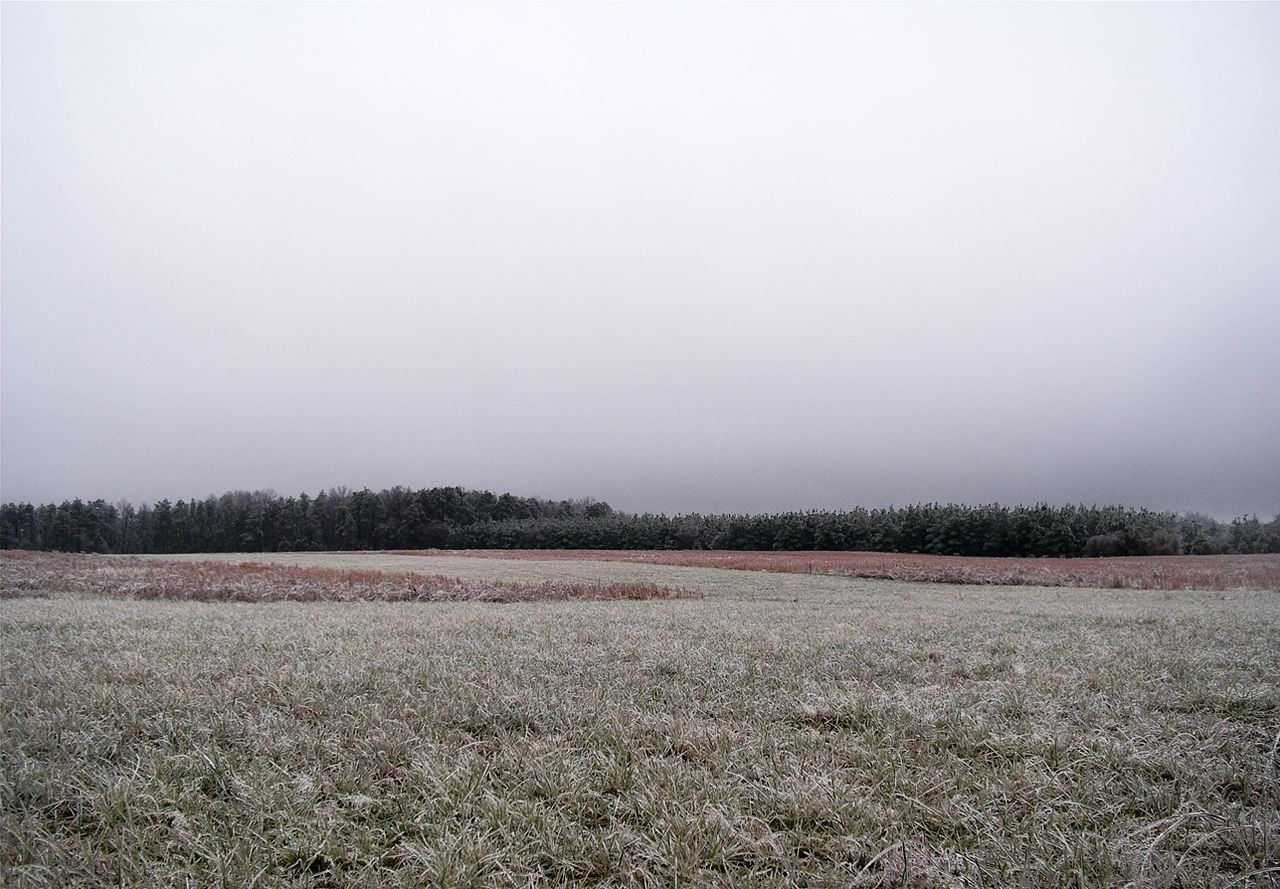
\includegraphics[width=\linewidth]{cloudforms-stratus}
            \captionof{figure}{Photographic reference of stratus clouds \protect\cite{img:cloudforms:stratus}.}
            \label{img:photo:cloudforms-stratus}        
        \end{minipage}        
    \hfill
        \begin{minipage}{0.47\linewidth}
            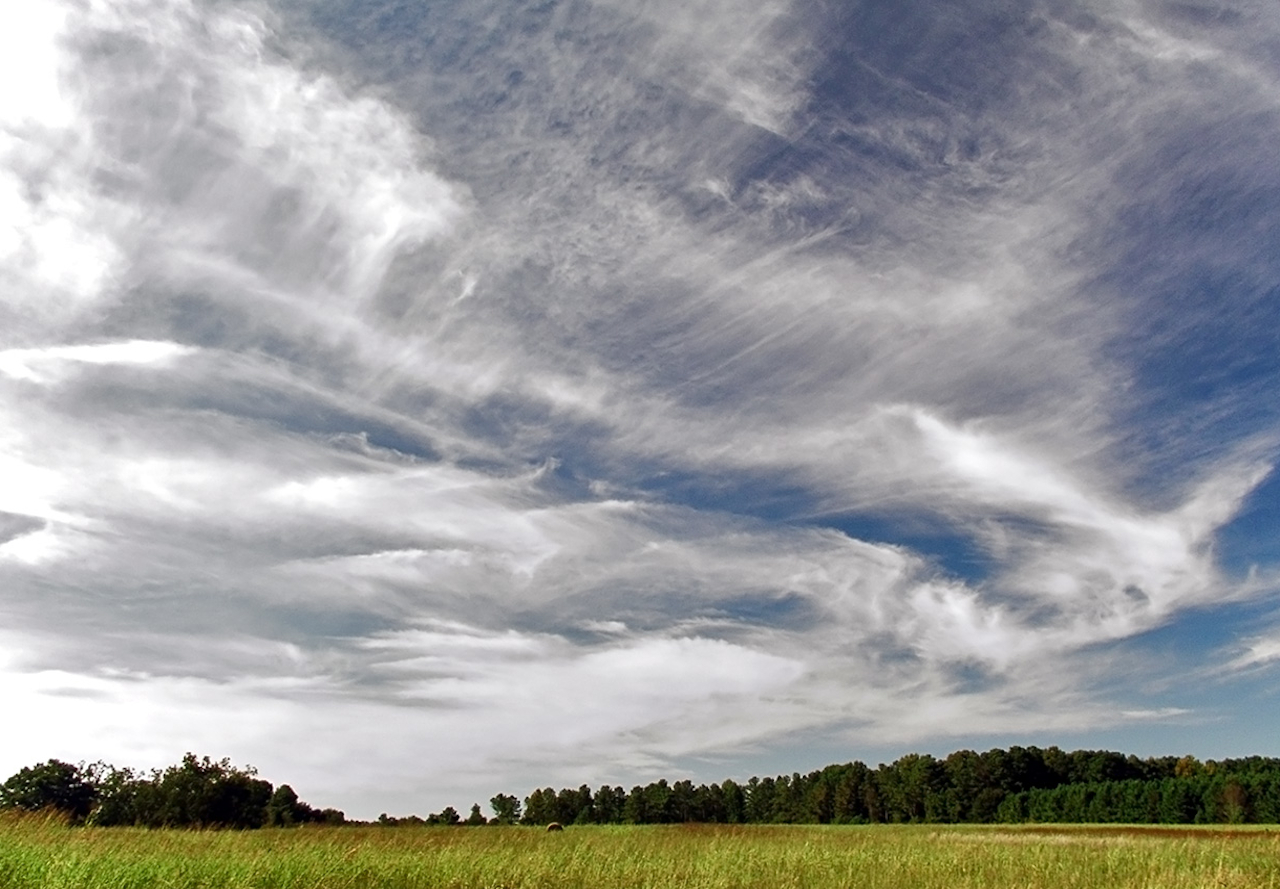
\includegraphics[width=\linewidth]{cloudforms-cirrus}
            \captionof{figure}{Photographic reference of cirrus clouds \protect\cite{img:cloudforms:cirrus}.}
            \label{img:photo:cloudforms-cirrus}        
        \end{minipage}
\end{figure}

\begin{figure}[ht]
    \centering
        \begin{minipage}{0.47\linewidth}
            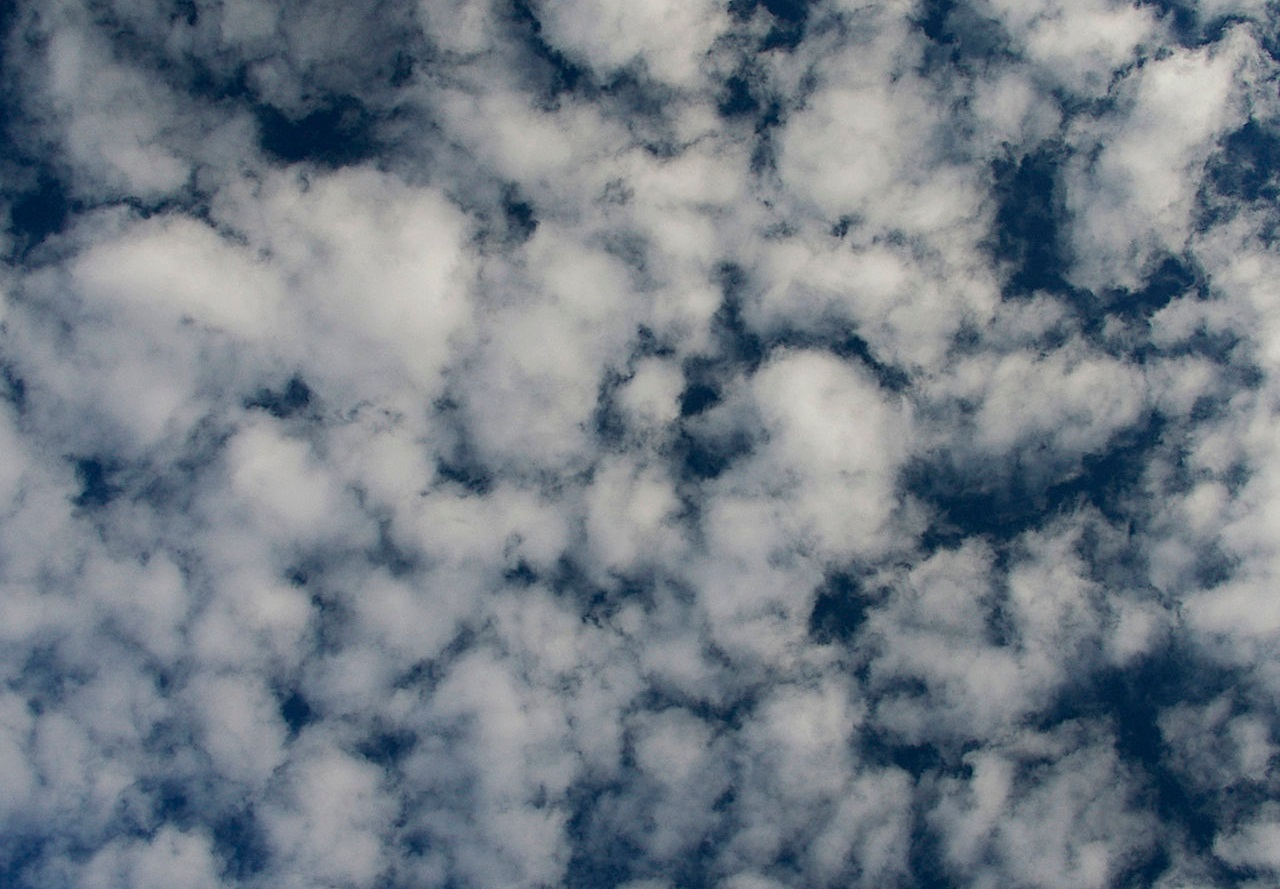
\includegraphics[width=\linewidth]{cloudforms-altocumulus}
            \captionof{figure}{Photographic reference of an altocumulus cloud formation \protect\cite{img:cloudforms:altocumulus}.}
            \label{img:photo:cloudforms-altocumulus}        
        \end{minipage}        
    \hfill
        \begin{minipage}{0.47\linewidth}
            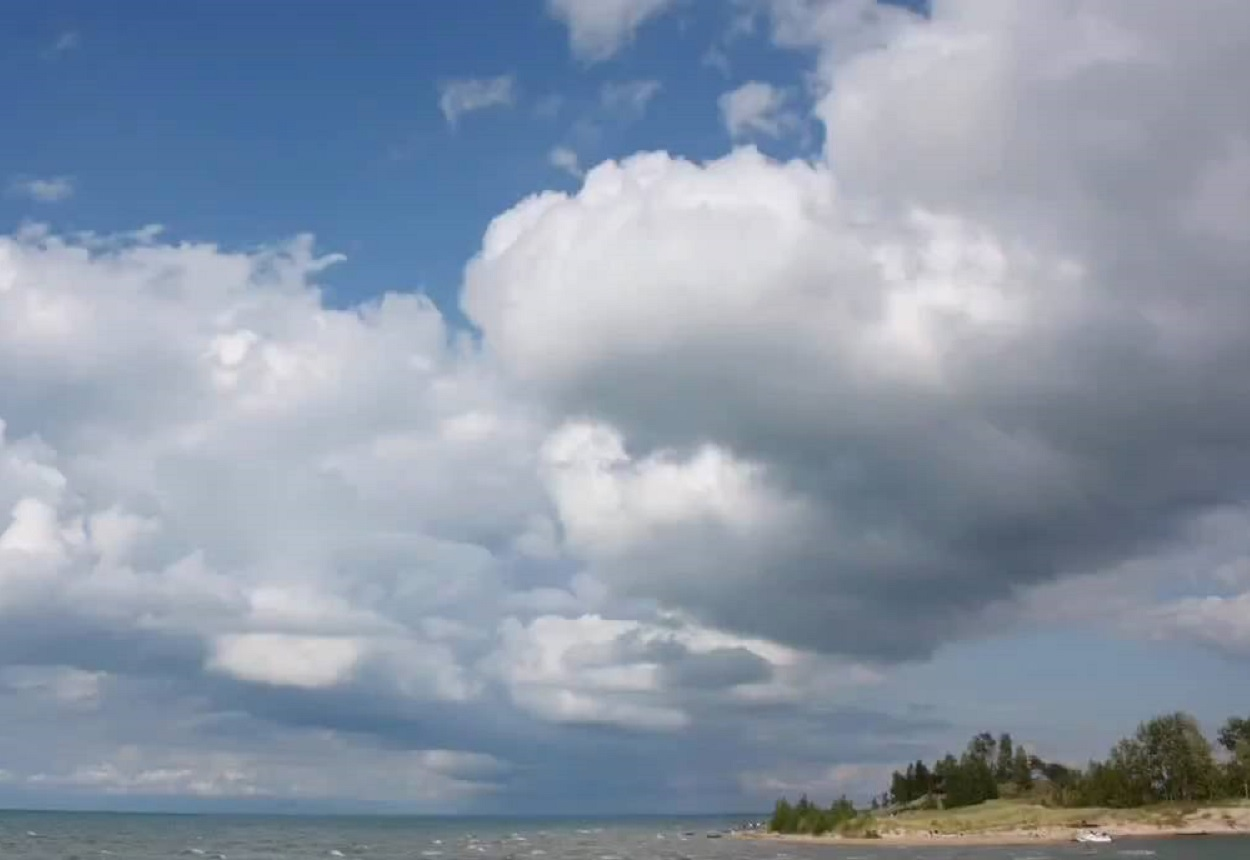
\includegraphics[width=\linewidth]{cloudforms-stratocumulus}
            \captionof{figure}{Photographic reference of stratocumulus cloudscape \protect\cite{img:cloudforms:stratocumulus}.}
            \label{img:photo:cloudforms-stratocumulus}        
        \end{minipage}  
\end{figure}

\subsection{Clouds in Games}
\label{section:clouds-in-games}
Depicted in \autoref{img:photo:cloudforms-altocumulus} and \autoref{img:photo:cloudforms-stratocumulus} of \sectionref{section:cloud-types} are clouds of the genus \textit{cumulus}, which translated to English means \textit{heap} or \textit{pile}.
Their remarkable cotton-like look makes them easy to recognize, which is also why they are often used in games as a reference for "normal" clouds. 
That is also the reason why the prototypes will mainly revolve around this genus.
\\
In games, the formation as well as the natural composition are both irrelevant, as the clouds are essentially only used for cinematic ambience or as a medium to enhance the atmosphere. This leaves just the rendering technique and performance to worry about.

\subsubsection{Skyboxes}
A widespread solution for representing clouds in games is not rendering them separately at all, but instead using a set of polar sky dome images, also known as the skybox. This is a six-sided cube which is rendered around the whole game world. On each inward looking face of the cube, one of the sky dome images is displayed, creating a seamless sky around the inner side of the box.
\begin{figure}[H]
    \centering
        \begin{minipage}{0.47\linewidth}
            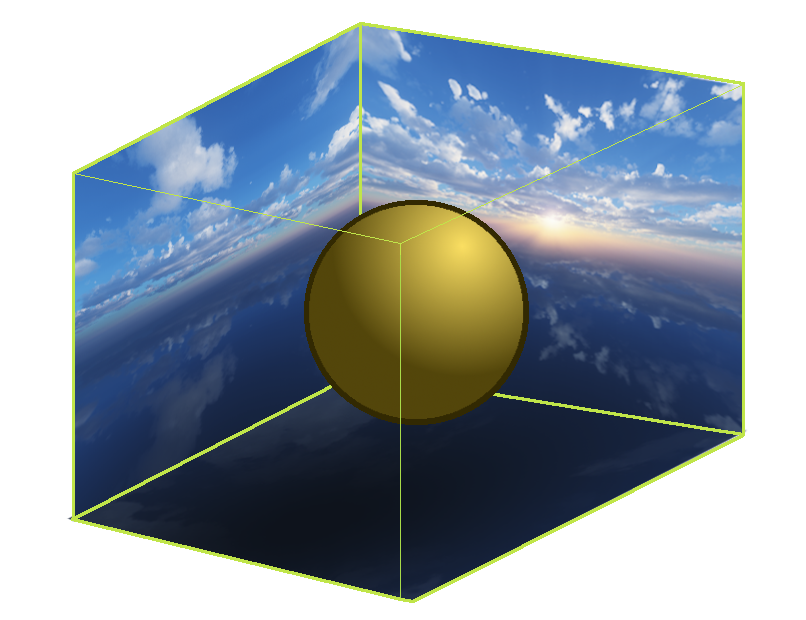
\includegraphics{edits/skybox}
            \captionof{figure}{The skybox cube as it is used in games.}
            \label{img:edits:skybox}
        \end{minipage}
    \hfill
        \begin{minipage}{0.45\linewidth}
            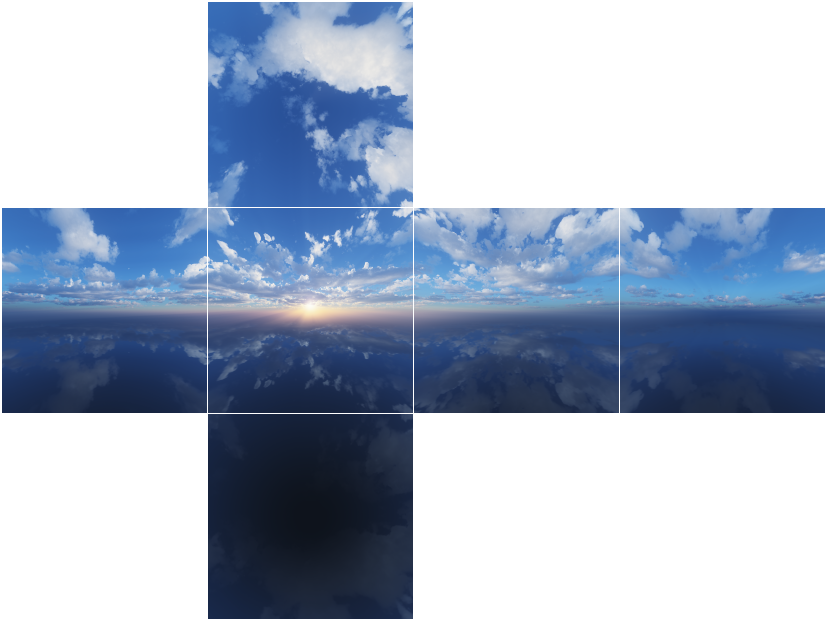
\includegraphics[width=\linewidth]{edits/skybox_layedout}
            \captionof{figure}{The polar sky dome images, folded out.}
            \label{img:edits:skybox_layedout}
        \end{minipage}
\end{figure}

\noindent
Besides rendering the sky, this of course allows clouds to be drawn right into the background. Also, in terms of performance, this is extremely cheap and efficient. On the other hand, it removes the ability for the clouds to move. 
They also have no volumetric body and no way of interaction with the game world whatsoever.
\\
This method does indeed give the scenery a more cloudy look, but what is missing is the "feel", or in other words the motion, interaction and lifelikeness of the clouds.

\subsubsection{Billboards}
Similar to the approach with the skybox, this technique also only uses 2D images of clouds. They are rendered individually and are always facing the camera. This is called \textit{\gls{billboard}ing}.
Now that each cloud is represented by its own game object, having a position in \gls{worldspace} as well as a scale and many other properties, it is possible to animate the clouds. For example, by moving the game objects in a circle around the world, the clouds seemingly "pass by".
\begin{figure}[H]
    \centering
        \begin{minipage}{0.48\linewidth}
            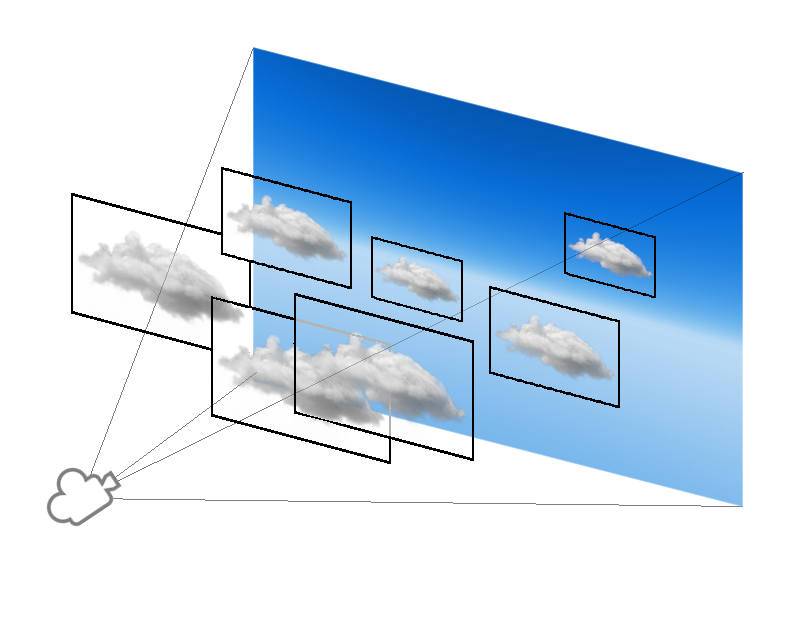
\includegraphics{edits/billboards}
            \captionof{figure}{A collection of 2D cloud billboards facing the camera.}
            \label{img:edits:billboards}
        \end{minipage}
    \hfill
        \begin{minipage}{0.45\linewidth}
            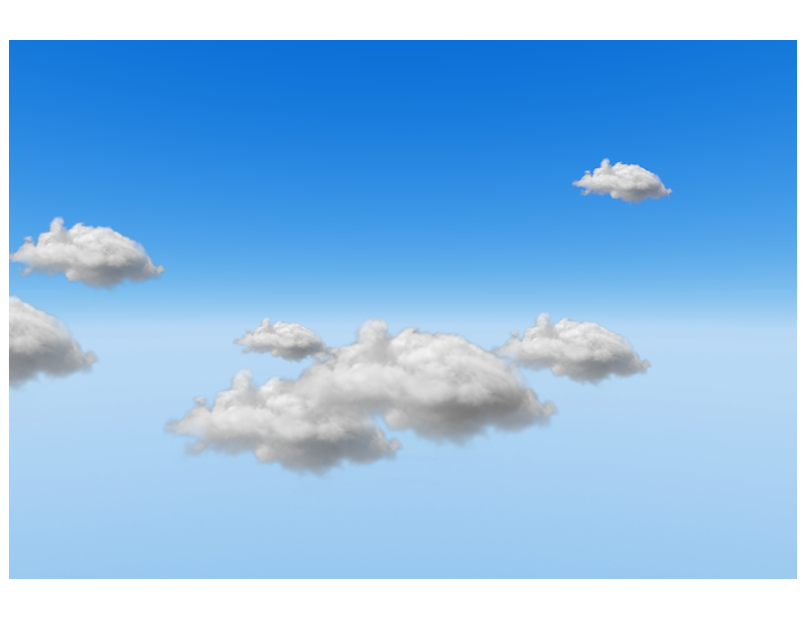
\includegraphics[width=\linewidth]{edits/billboards_rendered}
            \captionof{figure}{The rendered result of the image to the left.}
            \label{img:edits:billboards_rendered}
        \end{minipage}
\end{figure}
\noindent
Due to billboarding, the orientation is already given, making the overall time and effort of this technique quite advantageous to others.
\\
The major flaw of using billboards is of course that they are still 2D images, meaning they cannot really change appearance and therefore, do not evolve at all. 
Still, for many games, this technique suffices in the required diversity of background scenery and does not exceed the allowed performance share for such a task.

\subsubsection{Mesh-based Objects}
It is imaginable to simply use a \gls{polymesh} shaped like a cloud and render that like any other game object. By adding a texture, this would make for some decent looking clouds.
\\
However, the level of detail of such a polymesh is directly connected to the amount of vertices and faces that have to be processed every frame.
As seen in \autoref{img:rendered:cloud-mesh}, there are hundreds of polygons required to merely represent the basic shape of a realistic cloud.
If a similarly complex mesh is to be used for every cloud, a massive overhead is generated for objects that usually only contribute to the background of a game.
\begin{figure}[H]
    \centering
    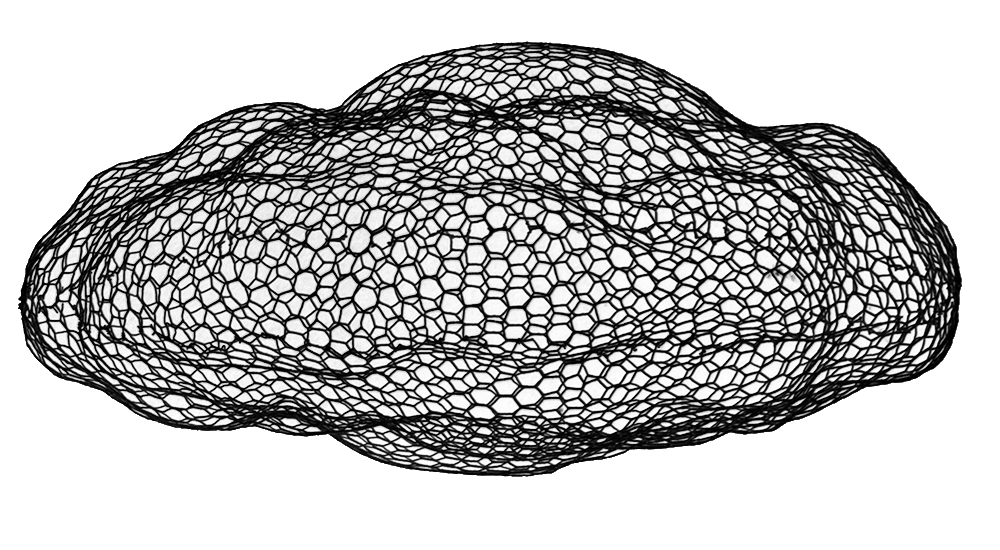
\includegraphics[width=0.5\linewidth]{rendered-cloud-mesh}
    \captionof{figure}{A \gls{polymesh} in the shape of an altocumulus cloud \cite{img:rendered:cloud-mesh}.}
    \label{img:rendered:cloud-mesh}
\end{figure}
\noindent
Apart from the performance impact, this method offers a volumetric, possibly interactable object just like any other 3D model does.
When massively decreasing the polygon count and therefore relinquishing the realistic look, mesh-based objects may be a viable solution for some \gls{lowpoly} games.
Otherwise, it is not reasonable to use this method.

\subsubsection{Volumetric Clouds}
Finally, clouds can be rendered via a technique called \textit{volumetric rendering}. The image below shows volumetric cloudscapes as seen in popular AAA titles.
The method itself is explained in detail in \sectionref{section:volumetric-rendering}.

\begin{figure}[H]
    \centering
    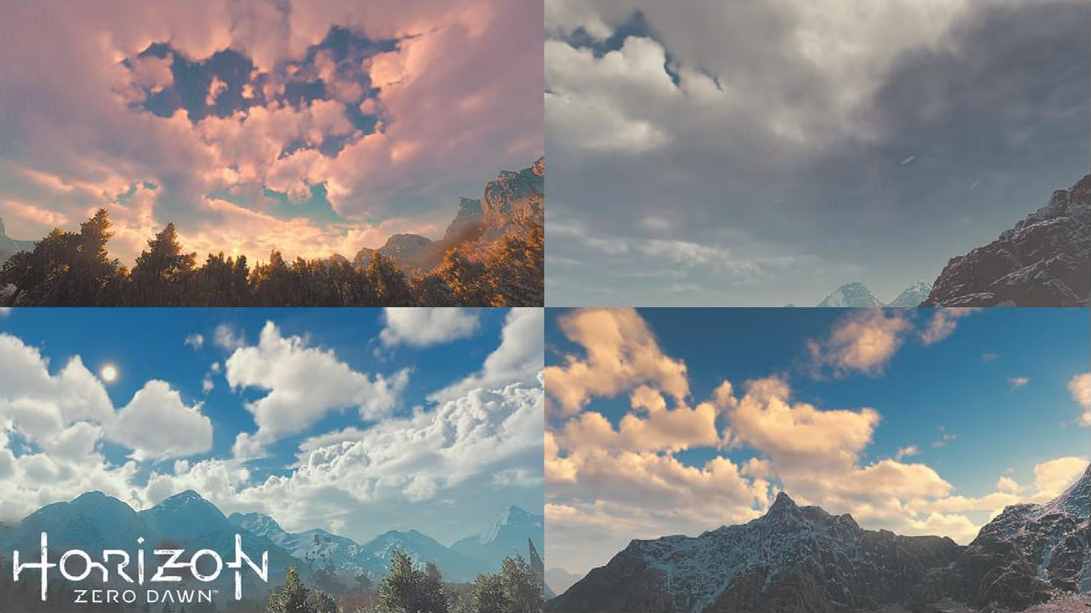
\includegraphics[width=\linewidth]{rendered-clouds-zerodawn}
    \captionof{figure}{Several volumetric cloudscapes from the game \textit{Horizon: Zero Dawn}, drawn in real time \protect\cite{img:rendered:clouds-zerodawn}.}
    \label{img:rendered:clouds-zerodawn}
\end{figure}